% beamer presentation template - rax 05.10.12
% main data
\def \ver {1.0}			% version number
\def \showver {0}		% 1 = show version/build; 0 = not show
\def \maintitle {Neuronal Connectivity via \\Bayesian Tensor Factorization}
\def \sbtitle {}
\def \shorttitle {Neuronal Connectivity via Tensor Factorization}
\def \lauthors {Chris Mulligan}
\def \sauthors {Chris Mulligan}
\def \presenter {}
\def \home {Columbia University}
\def \venue {Statistical Analysis of Neural Data}
\def \location {}
\def \ldate {December 15, 2015}

% ****************************************************************************
% Document Start
\documentclass[xcolor=svgnames]{beamer}

% **** packages ****
%\usepackage[english]{babel}
%\usepackage{rax_beamerpack}
%\usepackage{beamerthemeshadow}
%\usetheme{Columbia}
\newcommand{\tensor}[1]{
  \ensuremath{\underline{\mathbf{#1}}}}

% ****************************************************************************
% Document Data
\title[\shorttitle]{\maintitle}
\subtitle{\sbtitle}
\author[\sauthors]{\lauthors\\ \scriptsize{\em \home}}
\institute{\venue\\ \tiny{\location}}
\date[\sdate]{\scriptsize{\ldate}}

\usefonttheme{professionalfonts}

% ****************************************************************************
% ****************************************************************************
\begin{document}

%****************** Title Slide ******************
\begin{frame}[plain]
	\titlepage
\end{frame}

%****************** Document ******************
% *********************************************
\section{Neuron Network}
\begin{frame}{Neuronal Connections}
	There is significant interest in discovering and modeling connections
between neurons.

	General goal is to develop a directed graph of neuron connections. 

\end{frame}
\begin{frame}{Neuronal Connections}

	\begin{block}{Consider the standard setup:}
	Time series dataset of $y_{it}$, for $i=1,\ldots,N$ neurons over $t=1,\ldots,T$ time steps.

	$y_{it}$ is the number of times neuron $i$ fired at discrete time $t$ 
	\end{block}

	\begin{block}{Goal:}
	For each neuron $i$, infer the subset of neurons $j$ that either excite or inhibit neuron $i$. 
	\end{block}


\end{frame}

\begin{frame}{Neuronal Connections}
	\begin{block}{Lots of work in this space. A few examples:}
	\begin{itemize}
	\item Cross-Correlation based techniques
	\item Granger Causality
	\item $L_1$-regularized GLMs
	\item Factor Analysis
	\item Network Hawkes Processes
	\end{itemize}
	\end{block}
\end{frame}

% *********************************************
\section{Bayesian Tensor Factorization}
\begin{frame}{Consider Bayesian Tensor Factorization\footnote{Based on Schein, Paisley, Blei, and Wallach (2015)}}
	We consider using Bayesian tensor factorization as a means of inferring latent components that can be used to understand the relationships between neurons. \vspace{1em}

	Let $\tensor{Y}$ be a three way tensor of size $N \times N \times L$.

	$y_{ijl}$ is the count of times that neuron $i$ fired $l$ time steps after neuron $j$.


\end{frame}

\begin{frame}{Tensor Factorization}
	We use the Canonical Polyadic (CP) decomposition. The $K$ component decomposition decomposes the 3 way tensor into 3 latent factor matrices $\Theta^{(1)}, \Theta^{(3)}, \Theta^{(2)}$, with dimensions $d_m \times K$. 

	$$y_{ijl} \approx \hat{y}_{ijl} = \sum_{k=1}^K \theta^{1}_{ik} \theta^{2}_{jk} \theta^{3}_{lk}$$

	\begin{itemize}
	\item The columns of each of the $\Theta$ matrices represent a latent \textit{component}
	\item $\Theta^{(1)}_k$ vector represents the neurons being ``predicted''
	\item $\Theta^{(3)}_k$ represents the neurons being depended on
	\item $\Theta^{(2)}_k$ represents the lags of the dependency
	\end{itemize}
\end{frame}

\begin{frame}{Bayesian Tensor Factorization}
	View the tensor factorization probabilistically:
	$$y_{ijl} \sim Pois(\hat{y}_{ijl})$$

	Go Bayesian: impose priors on the latent factors. Gamma is conjugate to Poisson.

	Parameters: very small $a$ + small(ish) $b$. $\implies$ concentrate mass near 0, but heavy tail $\implies$ sparsity in the latent factors! 

	\begin{figure}[h]
	\centering
	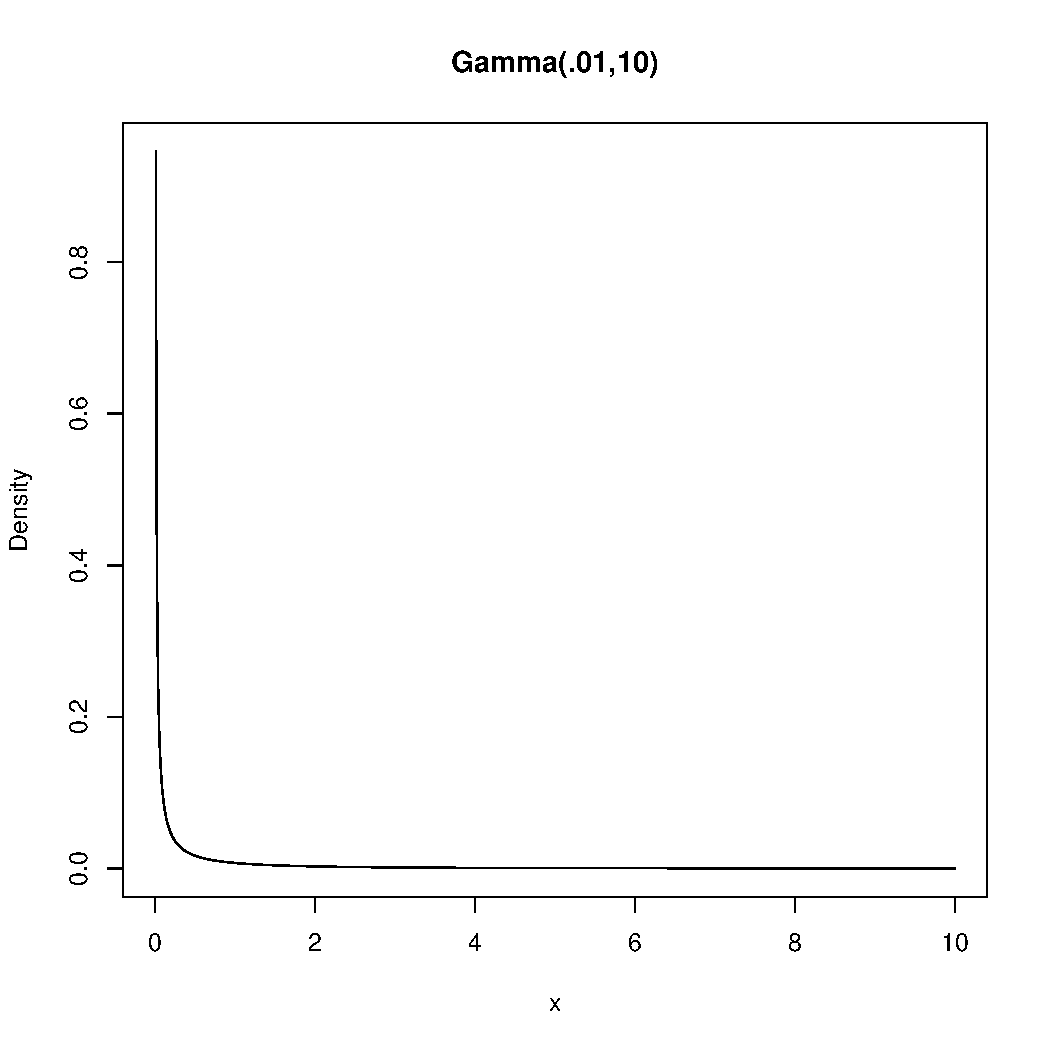
\includegraphics[width=.5\linewidth]{gamma}
	\caption{Gamma(.01, 10) Density}
	\end{figure}

\end{frame}

\begin{frame}{Approximate Inference}
	Posterior distribution: $P\left(\Theta^{(1:3)}, b \ |\  \tensor{Y}, a\right)$

	Must be approximated. Use variational inference with a mean field approximation, similar to what's commonly used in Bayesian Poisson Matrix Factorization. Use an independent Gamma for each latent factor, eg:

	$$P\left(\theta^{(1)}_{ik}|\cdot\right) \approx Q\left(\theta^{(1)}_{ik} | S^{(1)}_{ik}\right) = Gamma\left(\theta^{(1)}_{ik} | \alpha^{(1)}_{ik}, \beta^{(1)}_{ik}\right)$$

	Then choose $S^* = \textrm{argmin KL}(P || Q)$ via coordinate ascent, stopping when the ELBO converges. 
\end{frame}

% *********************************************
\section{Interpreting Results}
\begin{frame}{Interpreting Results}
	\begin{figure}[h]
	\centering
	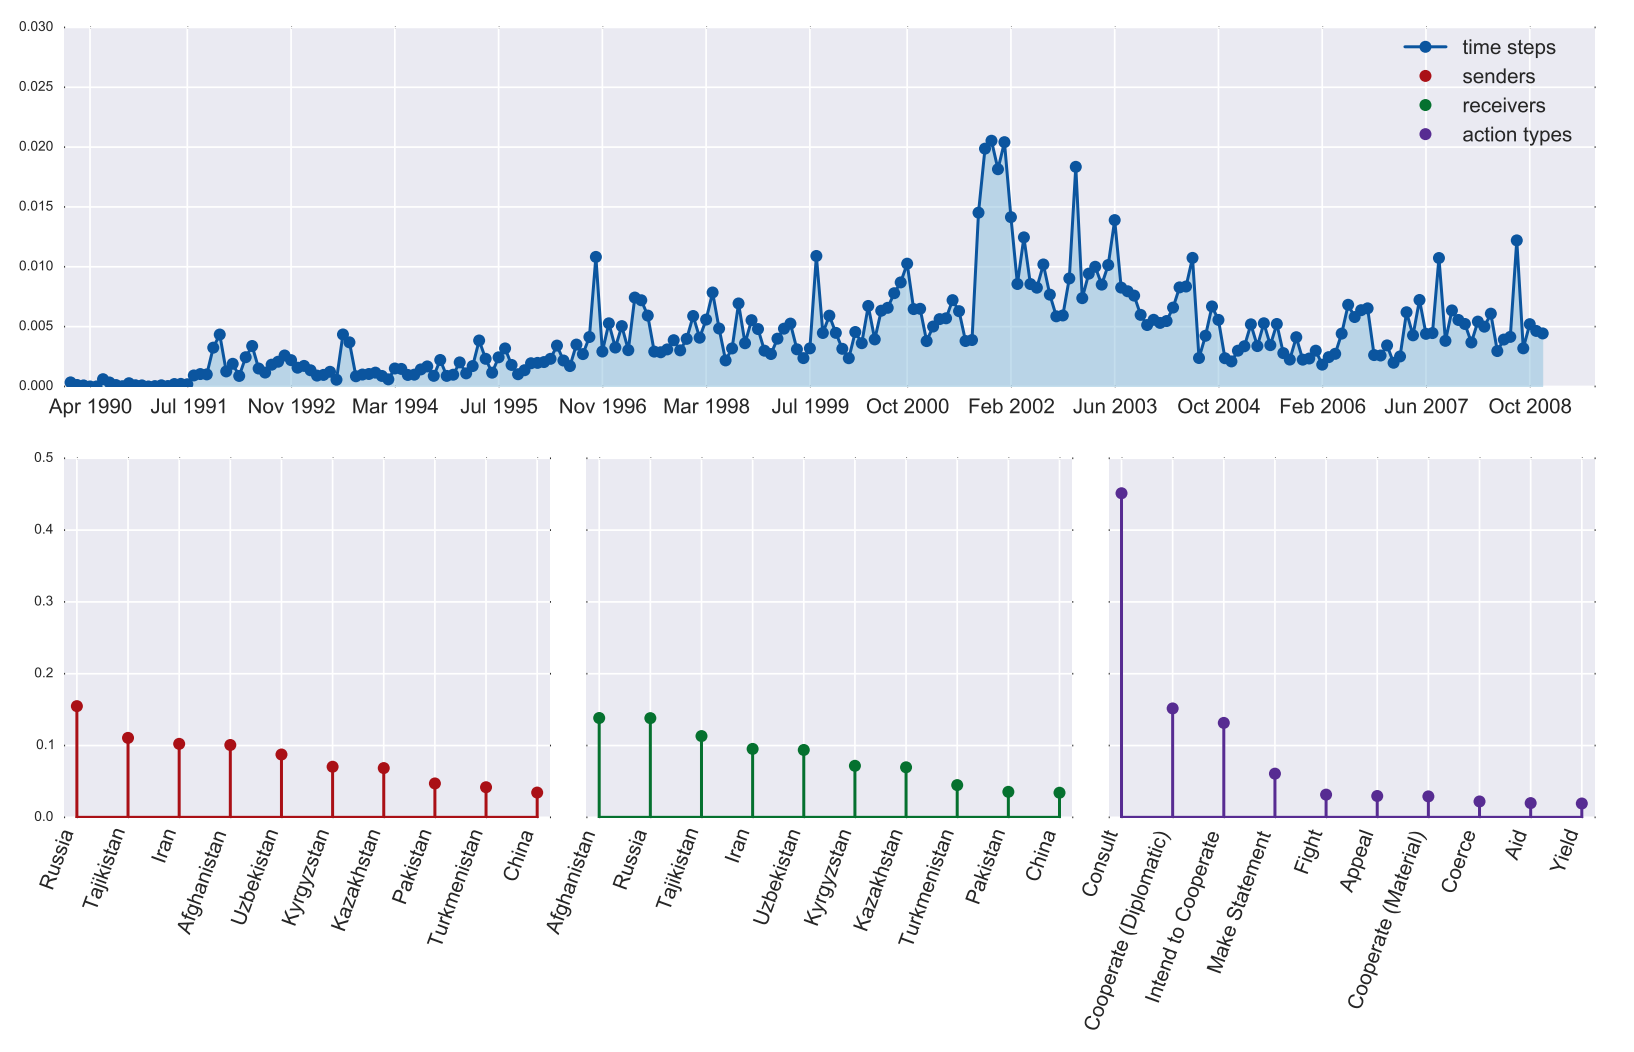
\includegraphics[width=\linewidth]{multilateral}
	\caption{One K component in Multilateral Relations from Schein et al}
	\end{figure}
\end{frame}

\begin{frame}{Interpreting Results 2}
	\begin{figure}[h]
	\centering
	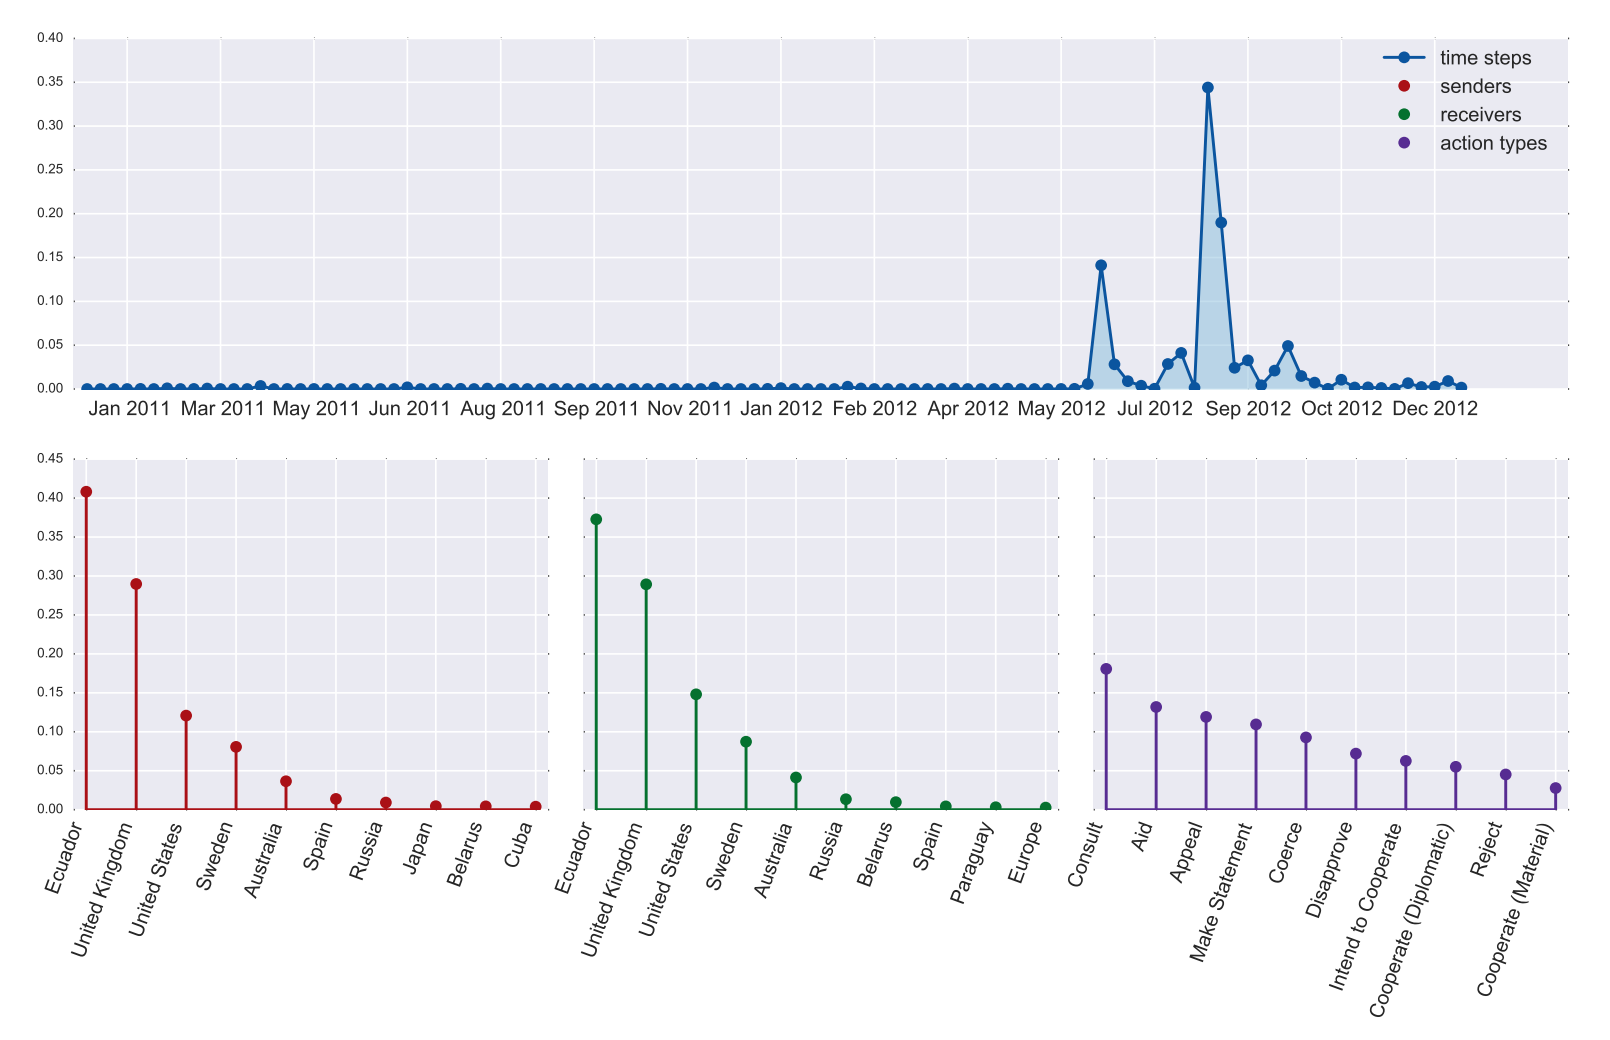
\includegraphics[width=\linewidth]{multilateral2}
	\caption{Another component: Wikileaks}
	\end{figure}
\end{frame}



\begin{frame}{Simple Synthetic Result}
	A small synthetic dataset consisting of 25 Neurons (with a few very strong connections) over 100,000ms was constructed with EnaS.

	The dataset was constructed with $L=20$ maximum lag, and fit with $K=6$ components.

	\begin{figure}[h]
	\centering
	\includegraphics[width=.5\linewidth,page=4]{../enas_sim1_raster_unit-time.out/45_trained_model.pdf}
	\caption{Component 3, which captures general neuron activity levels}
	\end{figure}
\end{frame}

\begin{frame}{Simple Synthetic Result}
	\begin{figure}[h]
	\centering
	\includegraphics[width=.65\linewidth,page=3]{../enas_sim1_raster_unit-time.out/45_trained_model.pdf}
	\caption{Component 2: Neuron 5 depends on Neuron 21, with a lag of 2}
	\end{figure}
\end{frame}

\begin{frame}{Simple Synthetic Result}
	\begin{figure}[h]
	\centering
	\includegraphics[width=.65\linewidth,page=2]{../enas_sim1_raster_unit-time.out/45_trained_model.pdf}
	\caption{Component 1: More complicated relationship, with a lag of 3}
	\end{figure}
\end{frame}

\begin{frame}{Simple Synthetic Result}
Several sensible ways of looking at the directed graph.

One is $\Theta^{(1)} \Theta^{(2)\textrm{T}}$, visualized below:
\begin{figure}[h]
	\centering
	\includegraphics[width=.65\linewidth,page=7]{../enas_sim1_raster_unit-time.out/45_trained_model.pdf}
	\end{figure}
\end{frame}


\begin{frame}{Connectomics Challenges Results}
	I used the Connectomics Challenge dataset. $N=100$ neurons, with $T\approx 180,000$. It's a highly clustered network. I deconvolved the fluorescence using PyFNND, which implements Voglestein et al.

	The dataset was constructed with $L=150$ maximum lag, and fit with $K=50$ components.

	\begin{figure}[h]
	\centering
	\includegraphics[width=.5\linewidth,page=4]{../fluorescence_iNet1_Size100_CC04inh.out/3_trained_model.pdf}
	\caption{Component 3, one of several which captures neuron correlations in ~time 0}
	\end{figure}
\end{frame}

\begin{frame}{Connectomics Challenges Results}\begin{figure}[h]
	\centering
	\includegraphics[width=.7\linewidth,page=4]{../fluorescence_iNet1_Size100_CC04inh.out/3_trained_model.pdf}
	\caption{3: one of several which captures neuron correlations in ~time 0}
	\end{figure}
\end{frame}


\begin{frame}{Connectomics Challenges Results}
\begin{figure}[h]
	\centering
	\includegraphics[width=.7\linewidth,page=32]{../fluorescence_iNet1_Size100_CC04inh.out/3_trained_model.pdf}
	\caption{31: Interesting temporal pattern, and sparse $i$ vector}
	\end{figure}
\end{frame}

\begin{frame}{Connectomics Challenges Results}
\begin{figure}[h]
	\centering
	\includegraphics[width=.7\linewidth,page=22]{../fluorescence_iNet1_Size100_CC04inh.out/3_trained_model.pdf}
	\caption{21: Note sparsity  of neurons, but relative flatness in time}
	\end{figure}
\end{frame}

\begin{frame}{Unfortunate Graph Results}
\begin{figure}[h]
	\centering
	\includegraphics[width=.4\linewidth,page=51]{../fluorescence_iNet1_Size100_CC04inh.out/3_trained_model.pdf}
	\hfill
	\includegraphics[width=.4\linewidth,page=1]{../network_iNet1_Size100_CC04inh.pdf}
	\caption{Left: Inferred with same method. Right: Actual}
\end{figure}
\end{frame}

%****************** Title Slide to Close ******************
% capture slide number to correct total number of slides later
\section{}
% clean background image if any
\begin{frame}
	  \centering \Huge
  Thanks!
\end{frame}


\end{document}
